\documentclass[12pt,a4paper]{report}
\usepackage{todonotes}

\usepackage[utf8]{inputenc} % pentru suport diacritice
\usepackage[romanian]{babel} % setări pentru limba română 
\renewcommand\familydefault{\sfdefault} % sans serif

\usepackage[margin=2.54cm]{geometry}	% dimensiuni pagină și margini
\usepackage{graphicx} % support the \includegraphics command and options

% formatting sections and subsections
\usepackage{textcase}
\usepackage[titletoc, title]{appendix}
\usepackage{titlesec}
\titleformat{\chapter}{\large\bfseries}{\thechapter}{2ex}{}[\vspace*{-1.5cm}]
\titleformat*{\section}{\large\bfseries}
\titleformat*{\subsection}{\large\bfseries}
\titleformat*{\subsubsection}{\large\bfseries}

\usepackage{chngcntr}
\counterwithout{figure}{chapter} % no chapter number in figure labels
\counterwithout{table}{chapter} % no chapter number in table labels
\counterwithout{equation}{chapter} % no chapter number in equation labels

\usepackage{booktabs} % for much better looking tables
\usepackage{url} % Useful for inserting web links nicely
\usepackage[bookmarks,unicode,hidelinks]{hyperref}

\usepackage{array} % for better arrays (eg matrices) in maths
\usepackage{paralist} % very flexible & customisable lists (eg. enumerate/itemize, etc.)
\usepackage{verbatim} % adds environment for commenting out blocks of text & for better verbatim
\usepackage{subfig} % make it possible to include more than one captioned figure/table in a single float
\usepackage{enumitem}
\setlist{noitemsep}

%%% HEADERS & FOOTERS
\usepackage{fancyhdr}
\pagestyle{empty}
\renewcommand{\headrulewidth}{0pt}
\renewcommand{\footrulewidth}{0pt}
\lhead{}\chead{}\rhead{}
\lfoot{}\cfoot{\thepage}\rfoot{}


\newcommand{\HeaderLineSpace}{-0.5cm}
\newcommand{\UniTextRO}{UNIVERSITATEA POLITEHNICA DIN BUCUREȘTI \\[\HeaderLineSpace] 
FACULTATEA DE AUTOMATICĂ ȘI CALCULATOARE \\[\HeaderLineSpace]
DEPARTAMENTUL CALCULATOARE\\}
\newcommand{\DiplomaRO}{PROIECT DE DIPLOMĂ}
\newcommand{\AdvisorRO}{Coordonator științific:}
\newcommand{\BucRO}{BUCUREȘTI}

\newcommand{\UniTextEN}{UNIVERSITY POLITEHNICA OF BUCHAREST \\[\HeaderLineSpace]
FACULTY OF AUTOMATIC CONTROL AND COMPUTERS \\[\HeaderLineSpace]
COMPUTER SCIENCE DEPARTMENT\\}
\newcommand{\DiplomaEN}{DIPLOMA PROJECT}
\newcommand{\AdvisorEN}{Thesis advisor:}
\newcommand{\BucEN}{BUCHAREST}

\newcommand{\frontPage}[6]{
\begin{titlepage}
\begin{center}
{\Large #1}  % header (university, faculty, department)
\vspace{50pt}
\begin{tabular}{p{6cm}p{4cm}}

\includegraphics[scale=0.8]{pics/upb-logo.jpg} &
	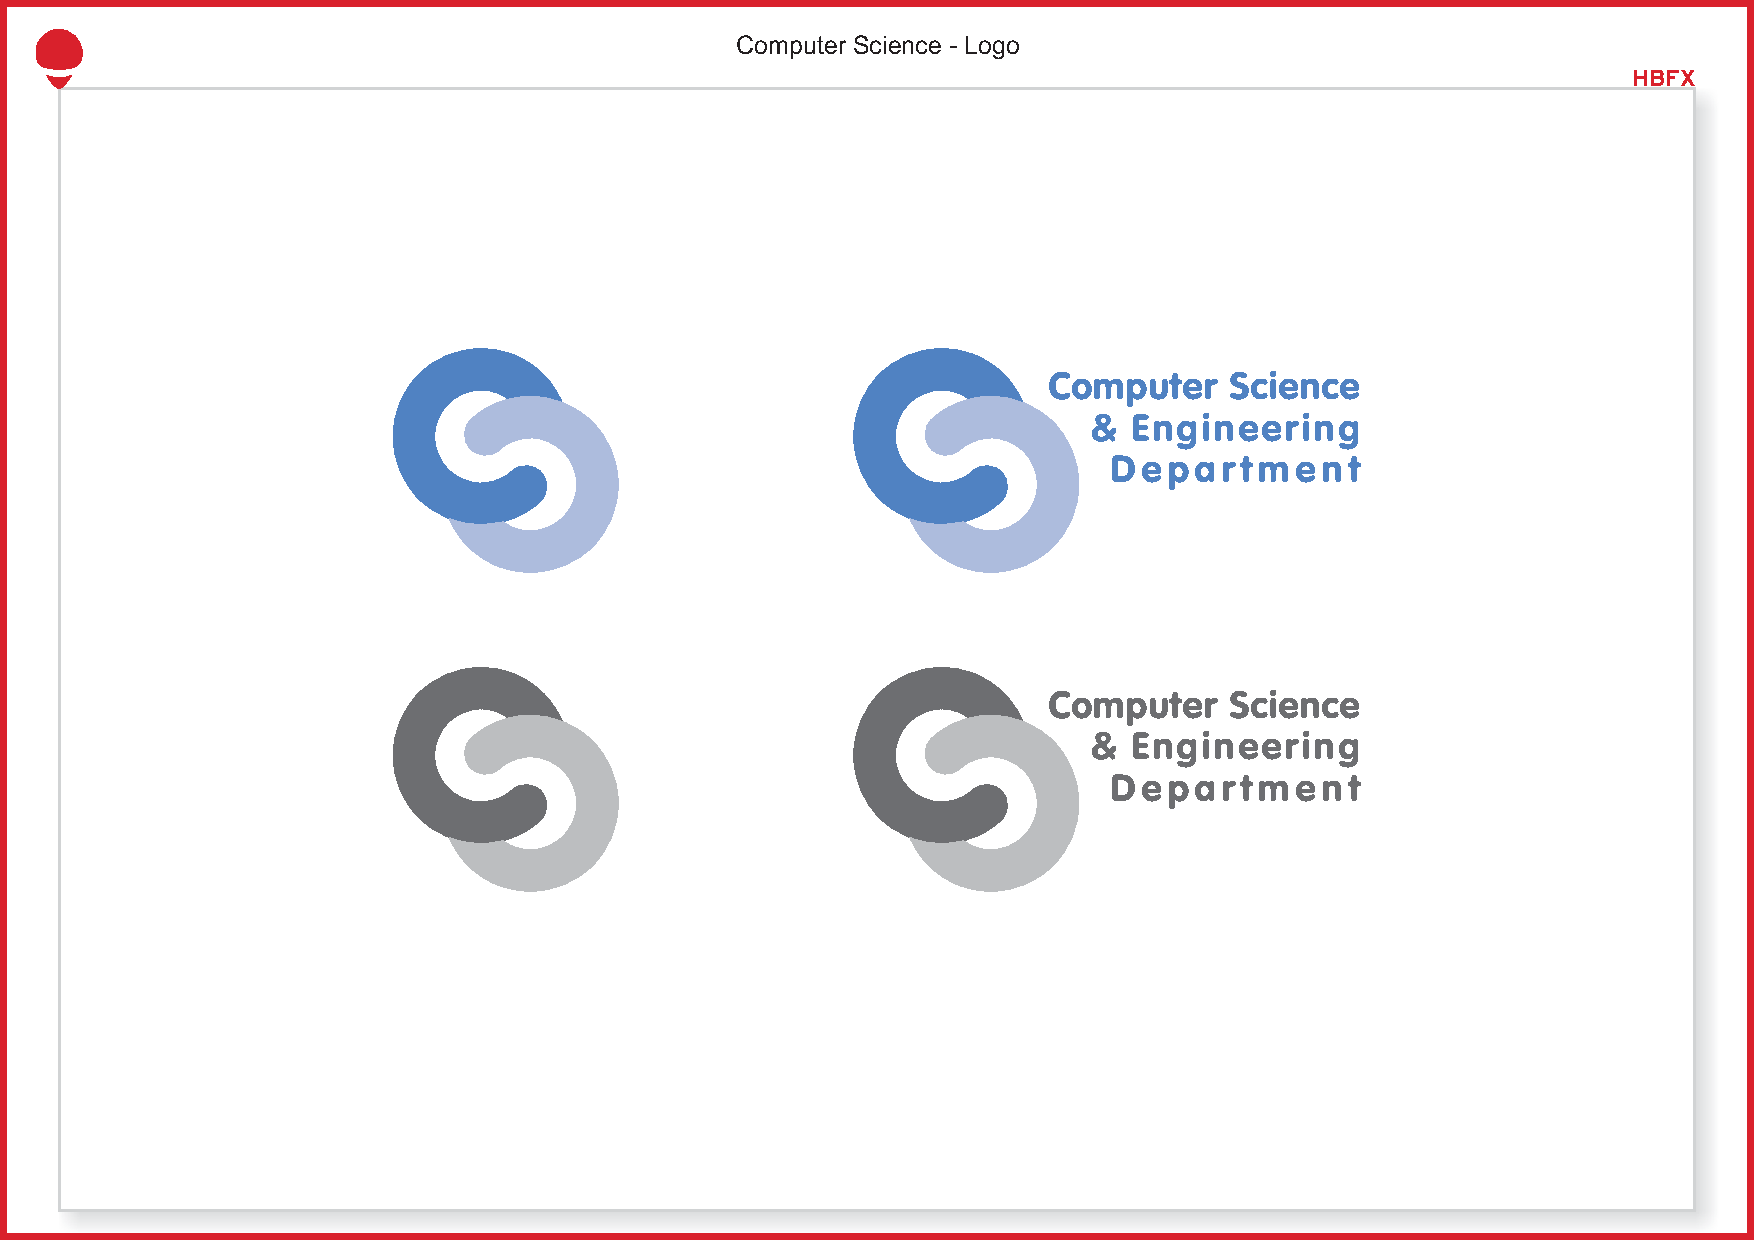
\includegraphics[scale=0.5,trim={14cm 11cm 2cm 5cm},clip=true]{pics/cs-logo.pdf}
\end{tabular}

\vspace{105pt}
{\Huge #2}\\                           % diploma project text
\vspace{40pt}
{\Large #3}\\ \vspace{0pt}  % project title
{\Large #4}\\                          % project subtitle
\vspace{40pt}
{\LARGE \Name}\\                   % student name
\end{center}
\vspace{60pt}
\begin{tabular*}{\textwidth}{@{\extracolsep{\fill}}p{6cm}r}
&{\large\textbf{#5}}\vspace{10pt}\\      % scientific advisor
&{\large \Advisor}                                    % advisor name
\end{tabular*}
\vspace{20pt}
\begin{center}
{\large\textbf{#6}}\\                                % bucharest
\vspace{0pt}
{\normalsize \Year}
\end{center}
\end{titlepage}
}

\newcommand{\frontPageRO}{\frontPage{\UniTextRO}{\DiplomaRO}{\ProjectTitleRO}{\ProjectSubtitleRO}{\AdvisorRO}{\BucRO}}
\newcommand{\frontPageEN}{\frontPage{\UniTextEN}{\DiplomaEN}{\ProjectTitleEN}{\ProjectSubtitleEN}{\AdvisorEN}{\BucEN}}

\linespread{1.5}
\setlength\parindent{0pt}
\setlength\parskip{.28cm}

%% Abstract macro
\newcommand{\AbstractPage}{
\begin{titlepage}
\textbf{\large SINOPSIS}\par
\AbstractRO\par\vfill
\textbf{\large ABSTRACT}\par
\AbstractEN \vfill
\end{titlepage}
}

%% Thank you macro
\newcommand{\ThanksPage}{
\begin{titlepage}
{\noindent \large\textbf{MULȚUMIRI}}\\
\Thanks
\end{titlepage}
}



%%%%%%%%%%%%%%%%%%%%%%%%%%%%%%%%%%%%%%%%%%%%%%%%%%   
%%
%%          End of template definitions
%%   
%%%%%%%%%%%%%%%%%%%%%%%%%%%%%%%%%%%%%%%%%%%%%%%%%%


%%% Puteți elimina aceste linii din lucrare, servesc numai pentru template.
\newcommand{\worktype}[1]{[\textit{#1}] }
\newcommand{\dezvoltare}{\worktype{Dezvoltare de produs}}
\newcommand{\cercetare}{\worktype{Cercetare}}
\newcommand{\ambele}{\worktype{Ambele}}
%%%


%%
%%   Campurile de mai jos trebuie modificate de autor. Modificati doar continutul, nu si numele fiecarei definitii
%%
\newcommand{\ProjectTitleRO}{Yuna, antrenoarea ta virtuală}
\newcommand{\ProjectSubtitleRO}{2018 versiunea 1}
\newcommand{\ProjectTitleEN}{Yuna, your virtual coaching}
\newcommand{\ProjectSubtitleEN}{2018 version 1}
\newcommand{\Name}{Sibel-Leila Bechir}
\newcommand{\Advisor}{Prof. dr. ing. Florica Moldoveanu}
\newcommand{\Year}{2018}

% Setări document
\title{Proiect de diplomă}
\author{\Name}
\date{\Year}

%%
%%   Campurile aferente rezumatului
%%
\newcommand{\AbstractRO}{Sinopsisul proiectului are rol de introducere, conținând atât o descriere pe scurt a problemei abordate cât și o enumerare sumară a rezultatelor și a concluziilor. Se recomandă ca sinopsisul să fie redactat într-un limbaj accesibil unei persoane nefamiliarizate cu domeniul, dar în același timp destul de specific pentru a oferi rapid o vedere de ansamblu asupra proiectului prezentat.
Sinopsisul proiectului va fi redactat atât în română cât și în engleză. Ca dimensiunea recomandată aceasta secțiune va avea maxim 200 de cuvinte pentru fiecare variantă. Împreună, ambele variante se vor încadra într-o singură pagină.}

\newcommand{\AbstractEN}{The abstract has an introductory role and should engulf both a brief description of the issue at hand, as well as an overview of the obtained results and conclusions. The abstract should be formulated such that even somebody that is unfamiliar with the projects’ domain can grasp the objectives of the thesis while, at the same time, retaining a specificity level offering a bird’s eye view of the project.
The projects’ abstract will be elaborated in both Romanian and English. The recommended size for this section is limited to 200 words for each version. Together, both versions will fit in one page.}

%%
%%   Campurile aferente paginii de multumiri
%%
%% \newcommand{\Thanks}{(opțional) Aici puteți introduce o secțiunea specială de mulțumiri / acknowledgments. }

\begin{document}

%%
%%  Prima pagina in romana
%%
\frontPageRO

%%
%%  Prima pagina in engleza
%%
%% \frontPageEN

\begingroup
\linespread{1}
\tableofcontents
\endgroup


% poate fi comentata sau stearsa
%% \ThanksPage

% Textul licentei incepe de aici 
\newpage


%%
%%  Introducere
%%
\chapter{Introducere}

\pagestyle{fancy}

Antrenoarea viruala isi propune sa ajute persoanele aflate in perioada de recaperare a mobilitatii dupa un accident. 

Au existat studii in care s-a demonstrat ca o persoana se poate recupera mai repede in ritmul propriu fata de programul cu constrangeri oferit de centrul specializat de recuperare. 

La centrul de terapie timpul petrecut pe un anumit exercitiu este destul limitat astfel pacientul neputand sa petreaca timpul necesar lui pentru a simti ca il realizeaza corect

% Pacientul poate sa isi extinda timpul necesar pentru realizarea unui exercitiu fata de perioada destul de limitata oferita de programarea la centrul de terapie.

Un alt factor important este rusinea de a pune o intrebari de mai multe ori terapeutului sau persoanei indrumatoarea.

Obiectivul acestui proiect este de a ajuta pacientii aflati in perioada de recuperare prin imbunatatirea progresului prin intermediul unuimediu familiar, precum apartamentul propriu, fata de un mediu necunoscut cum ar fi centrul de recuperare. De asemenea, oferira libertatii de a alege perioada de timp in care se pot face aceste exercitii.

Pentru a se determina cat de bine pacientul exerseaza si cum evolueaza, antrenoarea virtuala, Yuna, va detecta miscarile utilizatorului prin intermediul dispozitivului periferic Kinect. In functie de miscarile utilizatorului, Yuna  va oferi un calificativ acestuia in a il indruma spre a continua exersarea acestui exercitiul sau trecerea la urmatorul nivel de dificulate.


%%
%%  Analiza cerintelor
%%

%%
%%  Studiu de piata
%%
\chapter{Studiu de Piață}

In momentul actual, exista mai multe aplicatii care prin interediul Kinectului ajuta oamenii sa se recupereze precum si mentinerea formei fizice. Cateva exemple in acest sens sunt:


\section{Recuperarea dupa un atac cerebral}

Cercetatorii din cadrul Microsoft Asia impreuna cu universitatea nationala din Seul au realizat trei aplicatii pentru recuperarea fizica a persoanelor carea au suferit un atac vascular cerebral. 

Acestia au implementat box-and-block test care poate ajuta la evaluarea coordonararii, dexteritatii si capacitatea activității nervoase superioare. Utilizatorii trebuie sa mute cuburi dintr-o parte in alta. Numarul cuburilor mutate va oferi posibilitatea specialistilor de a observa procesul pacientului.

\begin{figure}[th]
\centering
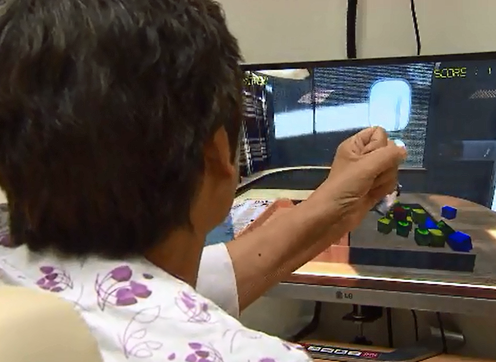
\includegraphics[width=0.6\columnwidth]{modele_existente/Box_and_Block_Stroke_Recovery.png}
  \caption[Box and Block Test]{Box and Block Test\protect\footnotemark}
  \label{figure_1:picture_2}
\end{figure}
\footnotetext{© https://www.microsoft.com/en-us/research/blog/stroke-recovery-gets-a-boost-from-kinect/}

Aceeasi cercetatori au dezvoltat pentru aceasi categorie de persoane o aplicatie in care participantii trebuie sa repete miscarile specialistului filmat. Acest exercitiu este inspirat din Fugl-Meyer Assessment.

Prin intermediul aplicatiei utilizatorul este mult mai relaxat in executarea miscarilor si perioada de recuperare poate reduce semnificativ.

\begin{figure}[th]
\centering
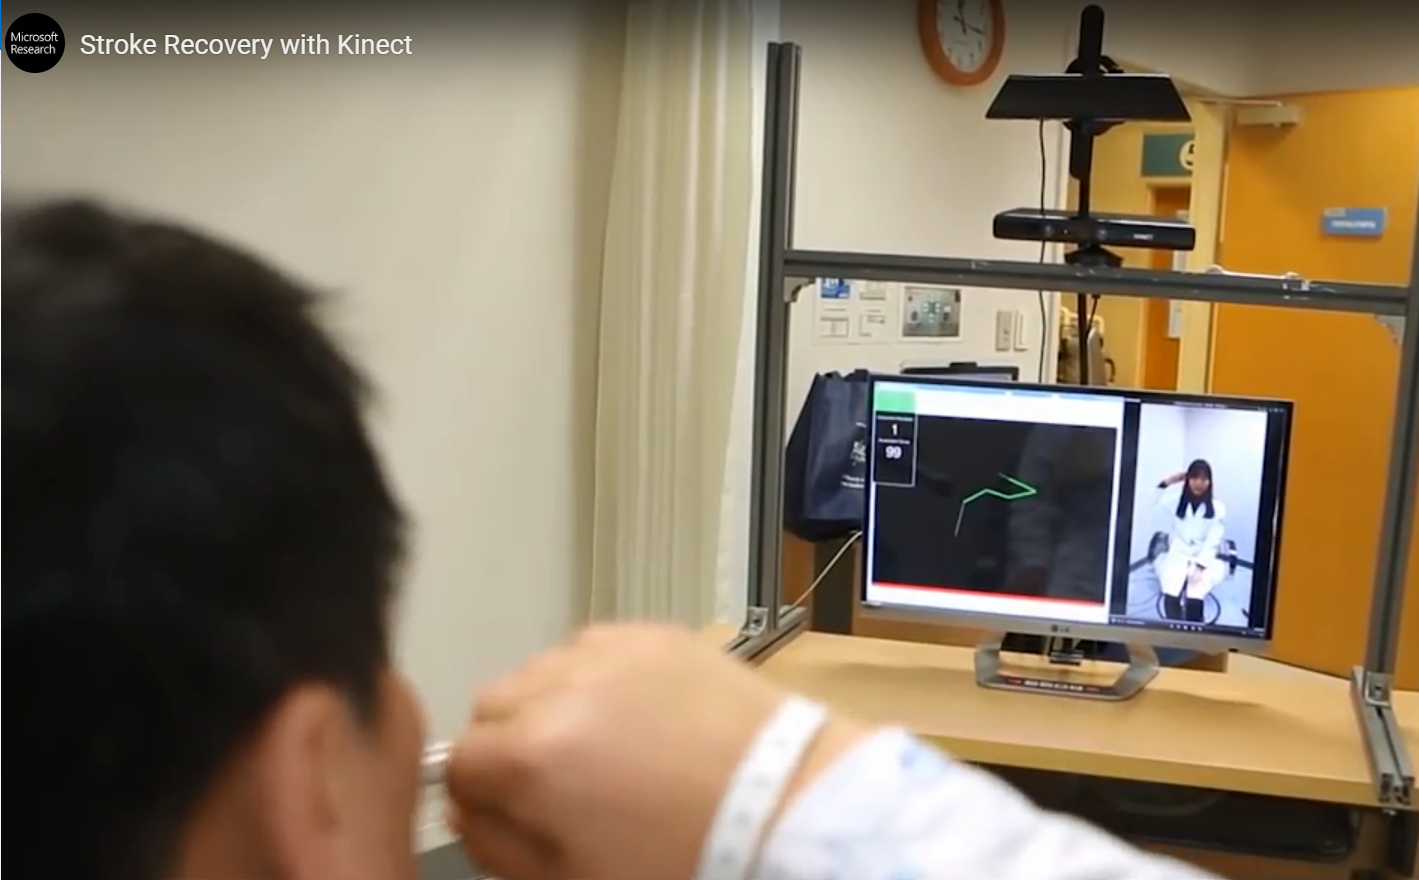
\includegraphics[width=0.6\columnwidth]{modele_existente/Fugl_Meyer_Assessment.png}
  \caption[Fugl-Meyer Assessment]{Fugl-Meyer Assessment\protect\footnotemark}
  \label{figure_1:picture_3}
\end{figure}
\footnotetext{© https://www.microsoft.com/en-us/research/blog/stroke-recovery-gets-a-boost-from-kinect/}

A treia aplicatie este cea in care pacienti isi pot exersa reactia si reflexia. Aceast aspect fiind determinat prin coliziunea dintre racheta condusa de ei si diferiti asteroizi. Miscarile rachetei sunt directionate de pozitia mainii relativ la umar.

\begin{figure}[th]
\centering
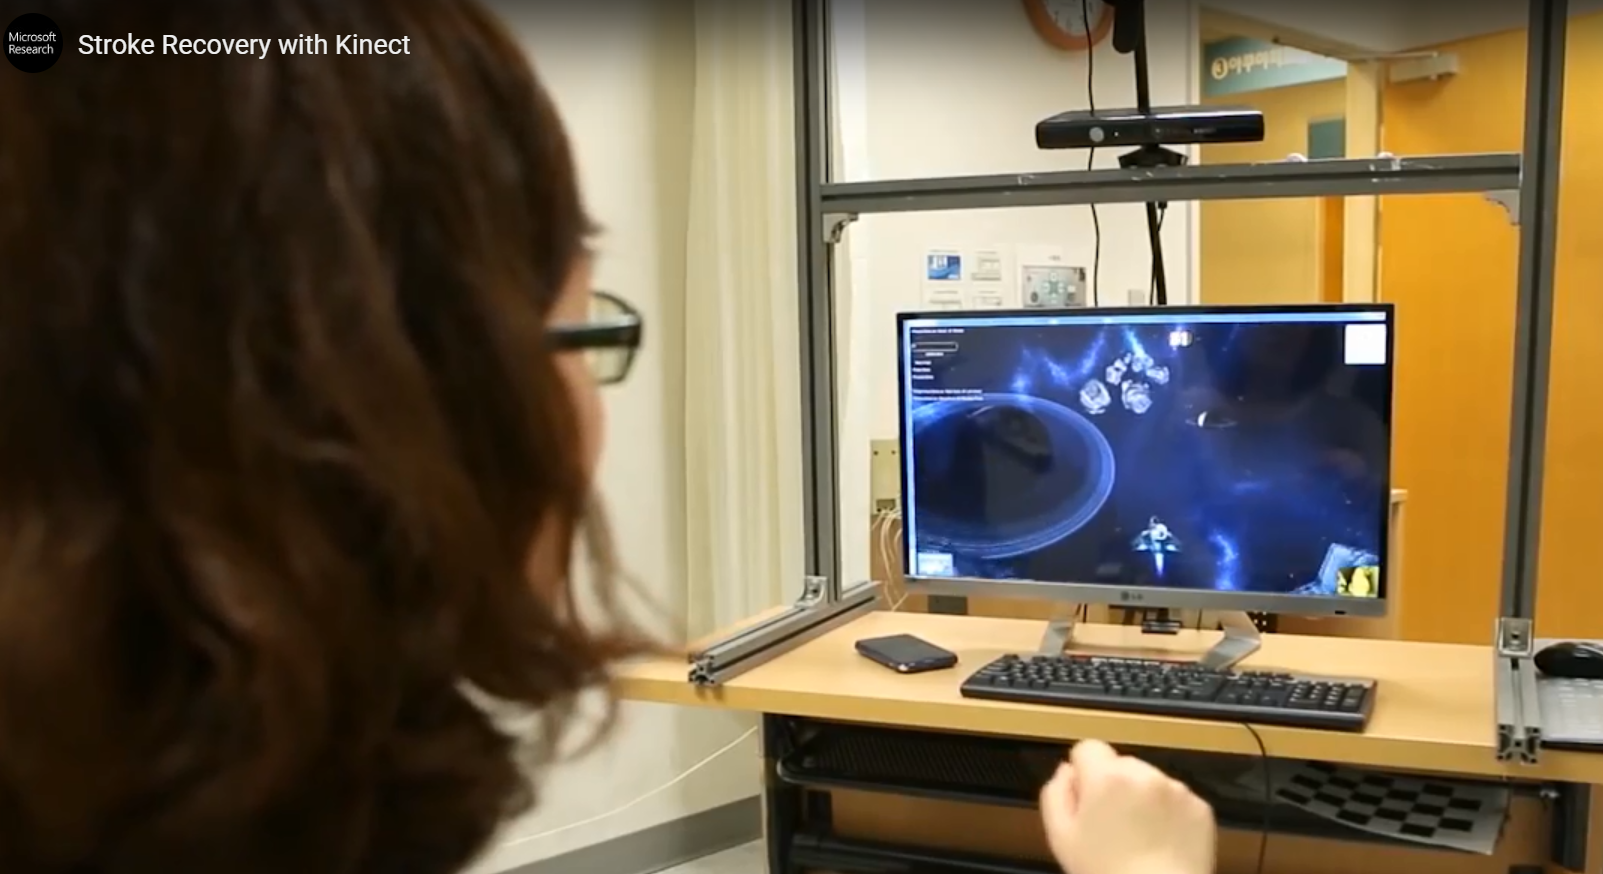
\includegraphics[width=0.6\columnwidth]{modele_existente/outer_space_game.png}
  \caption[Outer space game]{Outer space game\protect\footnotemark}
  \label{figure_1:picture_4}
\end{figure}
\footnotetext{© https://www.microsoft.com/en-us/research/blog/stroke-recovery-gets-a-boost-from-kinect/}

\section{The Biggest Loser: Ultimate Workout}

\textit{The Biggest Loser: Ultimate Workout} este o aplicatie implementa pentru Xbox 360 care cu ajutorul Kinect-ului ajuta utilizatorul sa slabeasca. Aceasta a fost inspirata din serialul televizat \textit{The Biggest Loser}. 

Exercitiile fizice sunt create astfel incat dificulatea sa fie direct proportionala cu evolutia jucatorului precum si particulrizate in functie de varsta si greutea utilizatorului. Contine peste 125 de exercitii si te poti antrene iar un bun element motivational este vocea antrenorilor.

\begin{figure}[th]
\centering
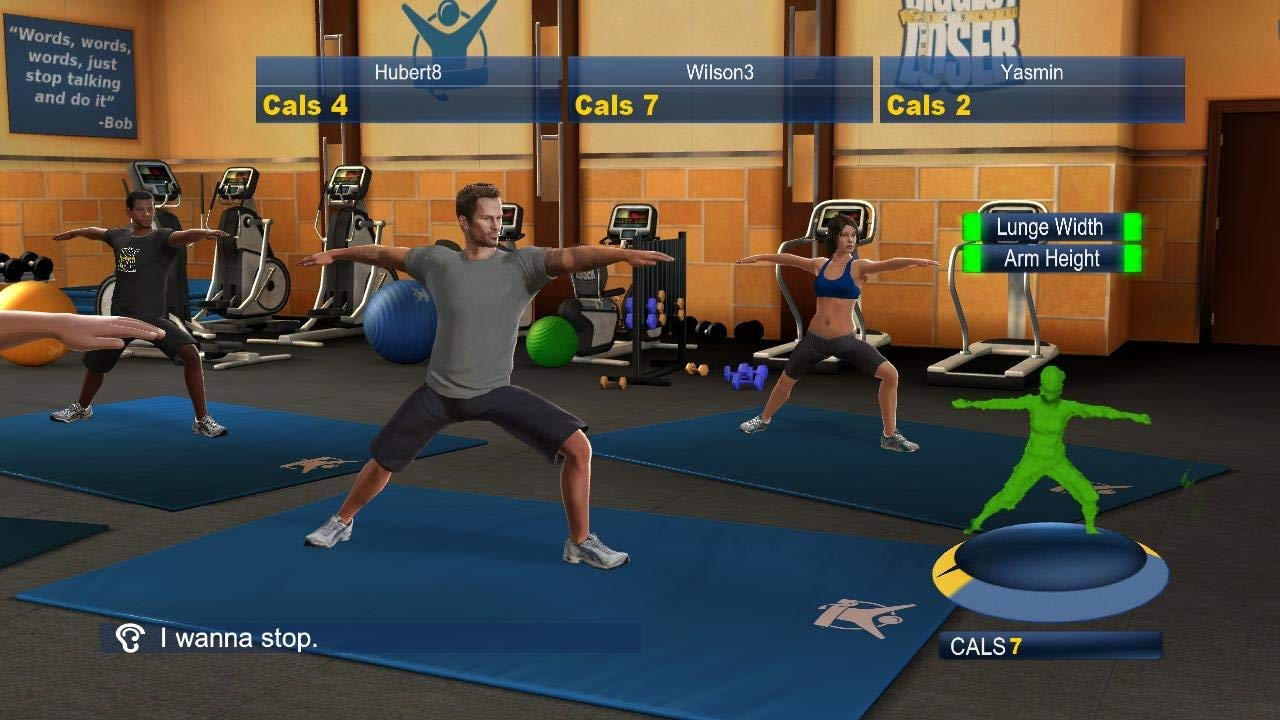
\includegraphics[width=0.6\columnwidth]{modele_existente/The_Biggest_Loser_Ultimate_Workout_Gameplay.jpg}
  \caption[The Biggest Loser Ultimate Workout gameplay]{The Biggest Loser Ultimate Workout gameplay\protect\footnotemark}
  \label{figure_1:picture_5}
\end{figure}
\footnotetext{© https://www.amazon.com/Biggest-Loser-Ultimate-Workout-Xbox-360/dp/B003S2SQFS}

% https://www.google.com/url?sa=i&source=images&cd=&ved=2ahUKEwjHrP_678rgAhUF6KQKHf0oCrsQjRx6BAgBEAU&url=http%3A%2F%2F123kinect.com%2Fkinect-games%2Fthe-biggest-loser-ultimate-workout%2F&psig=AOvVaw3ClV_tzvNqOKaknSJRw9hw&ust=1550771442698655

\section{EA Sports Active 2}

Aceasta aplicatie este dedicata firness-ului si contine 2 device-uri foarte importante care ajuta  in monitorizarea batailor inimii afisate pe ecran. 

Un aspect foarte interesant este dat de contul online al utilizatorului care contine toate antrenamentele, bataiile inimii, numarul de calorii arse precum si alte date importante din istoricul persoanei ceea ce duce la imbunatairea conditiei fizice.

\begin{figure}[th]
\centering
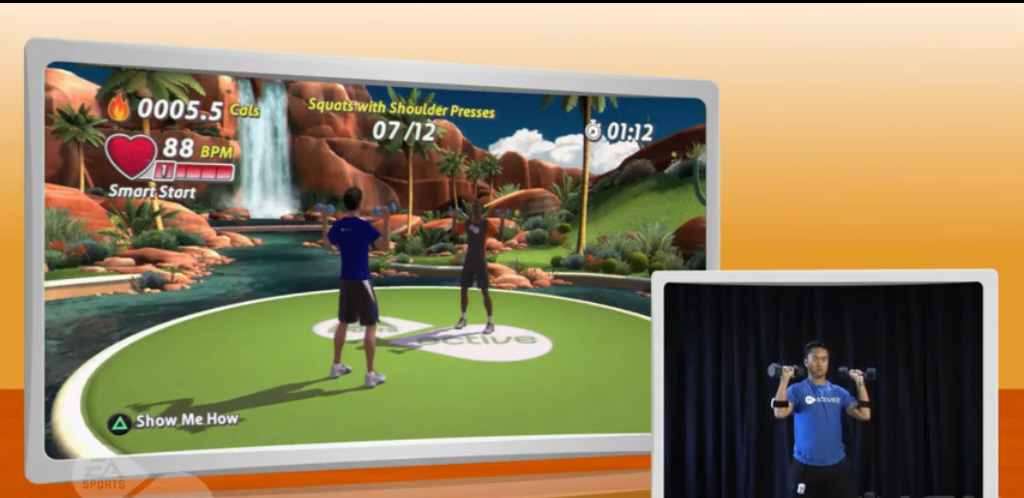
\includegraphics[width=0.7\columnwidth]{modele_existente/EA_Sports_Active_2_gameplay.jpg}
  \caption[EA Sports Active 2 Gameplay]{EA Sports Active 2 gameplay\protect\footnotemark}
  \label{figure_1:picture_6}
\end{figure}
\footnotetext{© https://www.videogamesblogger.com/2010/11/16/ea-sports-active-2-walkthrough-video-guide-xbox-360-ps3-wii.htm}

Prima versiune a fost pe Wii iar in urmatoarea versiune a fost lansata cu ajutorul Microsoft Kinect. In momentul actual EA Sports Active 2 suporta Wii, PlayStation 3 precum si Xbox 360.

%%\begin{figure}[th]
%%\centering
%%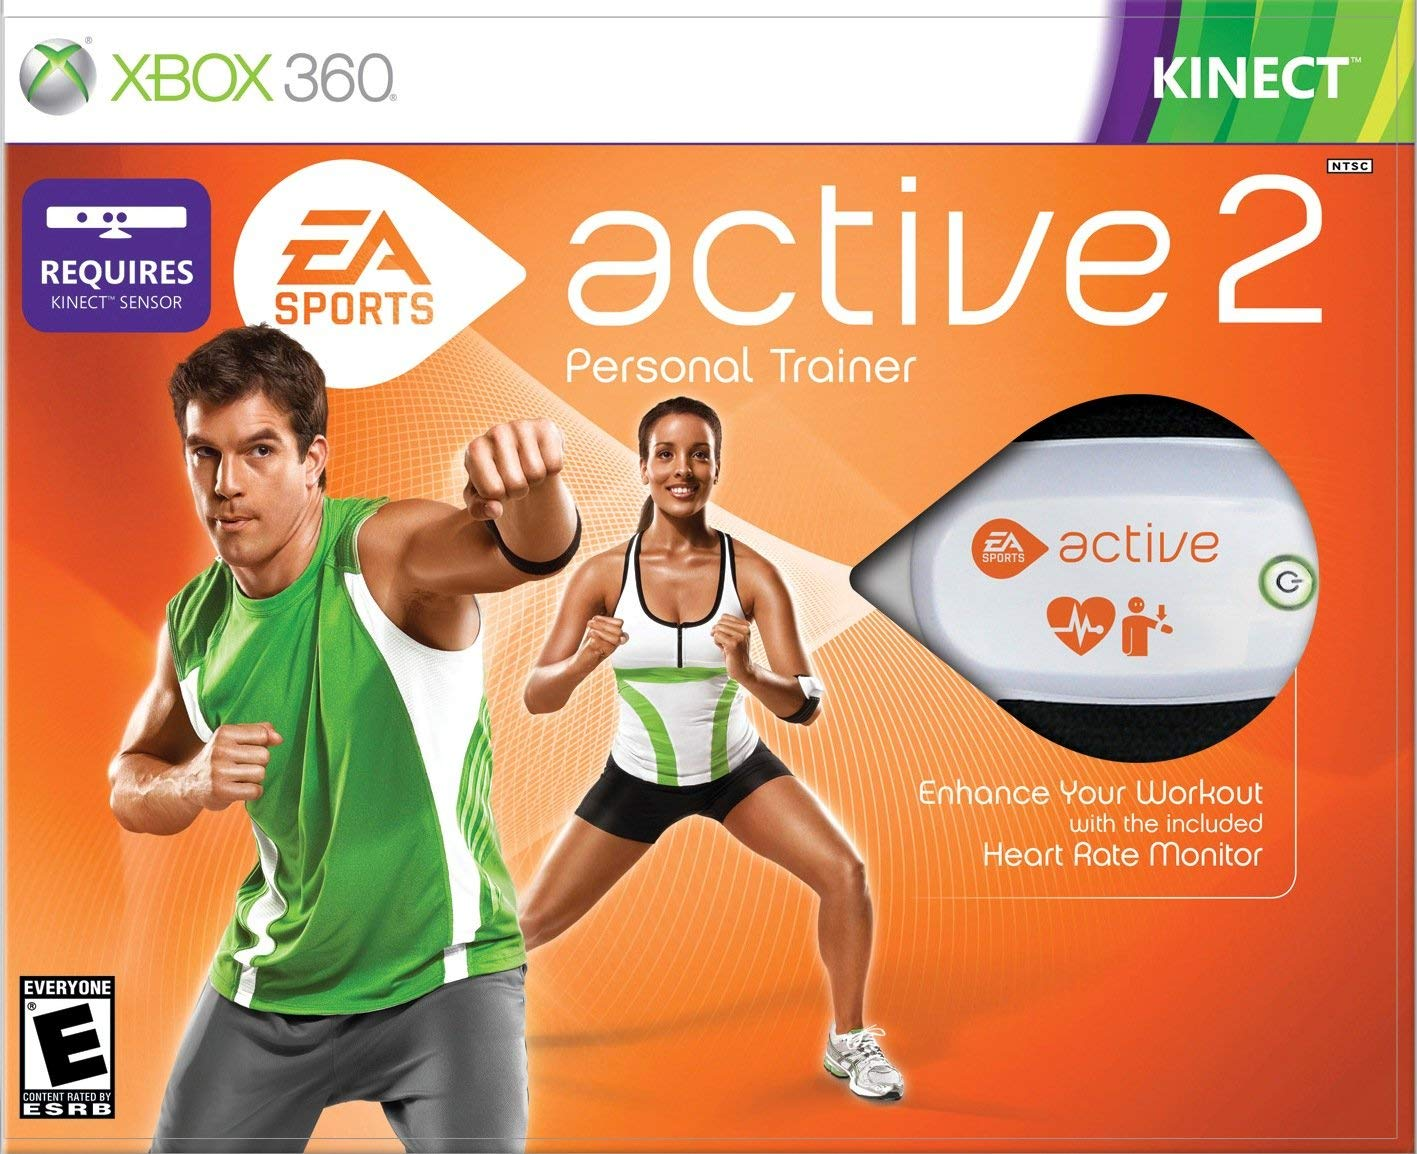
\includegraphics[width=0.4\columnwidth]{modele_existente/EA_Sports_Active_2.jpg}
%%  \caption[EA Sports Active 2]{EA Sports Active 2\protect\footnotemark}
%%  \label{figure_1:picture_7}
%%\end{figure}
%%\footnotetext{© https://images-na.ssl-images-amazon.com/images/}
%%
% https://images-na.ssl-images-amazon.com/images/I/81cgo-6RGzL._AC_SL1417_.jpg

\section{Zumba Fitness Rush - Groove Yourself To Health}

Persoanele care folosesc Zumba Fitness isi mentin forma prin intermediul unor miscari de dans. Aplicatia contine 24 de stiluri internationale de dans oferind un tutorial pentru invatarea fiecarui pas de dans. 

De asemenea, ritmul este foarte alert oferindu-i antrenamentului un nivel ridicat de dificultate si efort. Exercitiile se pot face pe melodiile unor interpreti foarte cunoscuti precum Tiesto, Pitbull precum si alti artisti. 

Zumba Fitness Rush - Groove Yourself To Health a fost dezvoltata de Pipeworks Software si este disponibila pe Wii, PlayStation si Xbox.

\begin{figure}[th]
\centering
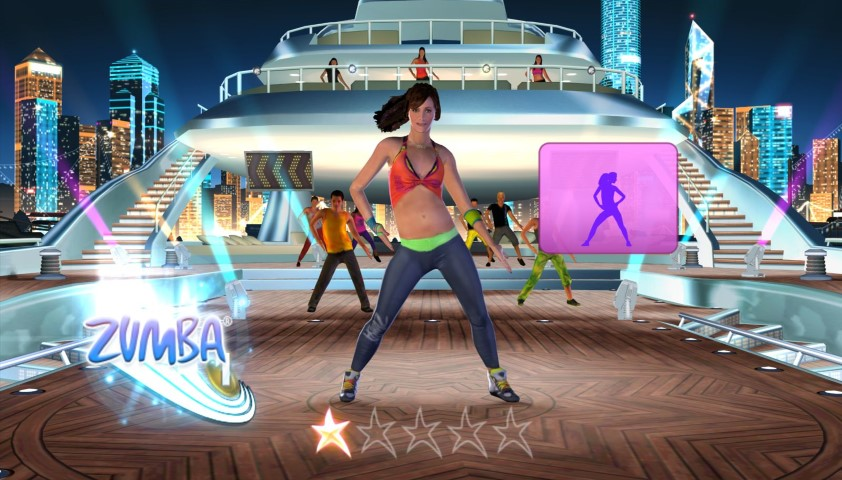
\includegraphics[width=0.6\columnwidth]{modele_existente/Zumba_Fitness.jpg} 
  \caption[Zumba Fitness]{Zumba Fitness\protect\footnotemark}
  \label{figure_1:picture_8}
\end{figure}
\footnotetext{© http://www.impulsegamer.com/360zumbafitnesscore.html}

\section{Shape Up}

Ubisoft a venit cu o un nou nivel pentru antrenamente. Acestea ofera un aspect mai amuzant in executaea miscarilor fizice precum si un timp mai scurt deorece utilizatorii se distreaza.

Un exemplu in acest sent sunt genoflexiunile deoarece cu cat utilizatorul executa mai multe cu atat acesta ajunge mai sus de pe pamant pe spatiu.

Cei din echipa Ubisoft a venit cu ideea de a ilustra obiecte din ce in ce mai mari cu cat se executa mai multe flotari. Acestea pornind de la valize la masini si la elefanti care sunt pozitionati pe spatele utilizatorului.

Aceasta aplicatie a fost creata de Ubisoft numai pentru Xbox One si a fost lansat in noiembrie 2014.

\begin{figure}[th]
\centering
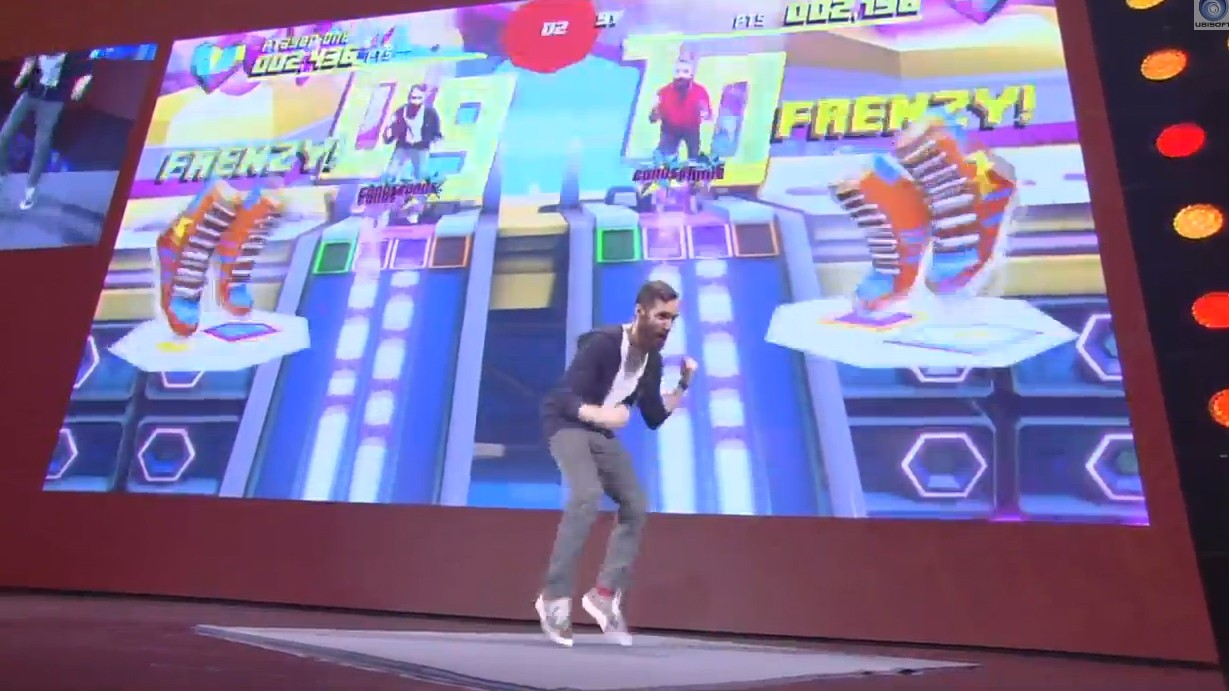
\includegraphics[width=0.6\columnwidth]{modele_existente/Shape_Up.jpg}
  \caption[Shape Up]{Shape Up\protect\footnotemark}
  \label{figure_1:picture_9}
\end{figure}
\footnotetext{© https://www.moddb.com/groups/anime/news/ubisoft-bets-wide}


%%
%%  Detalii de implementare
%%
\chapter{Detalii de implementare}

%%
%%  Crearea avatarului - MakeHuman
%%
\section{Crearea avatarului - MakeHuman}

Creatrea caracterului Yunei a fost realizat cu ajutorul software-ului open source de creare a humanoizilor tridimensionali, MakeHuman versiunea 1.1.1.

MakeHuman pune la dispozitie un humanoid care poate fi transformat fie in barbat sau femeie. Ca apoi sa il particularizezi mai mult ajutandu-ne de varsta, inaltime, culoarea pielii, forma fetei si forma corpului.

\begin{figure}[th]
\centering
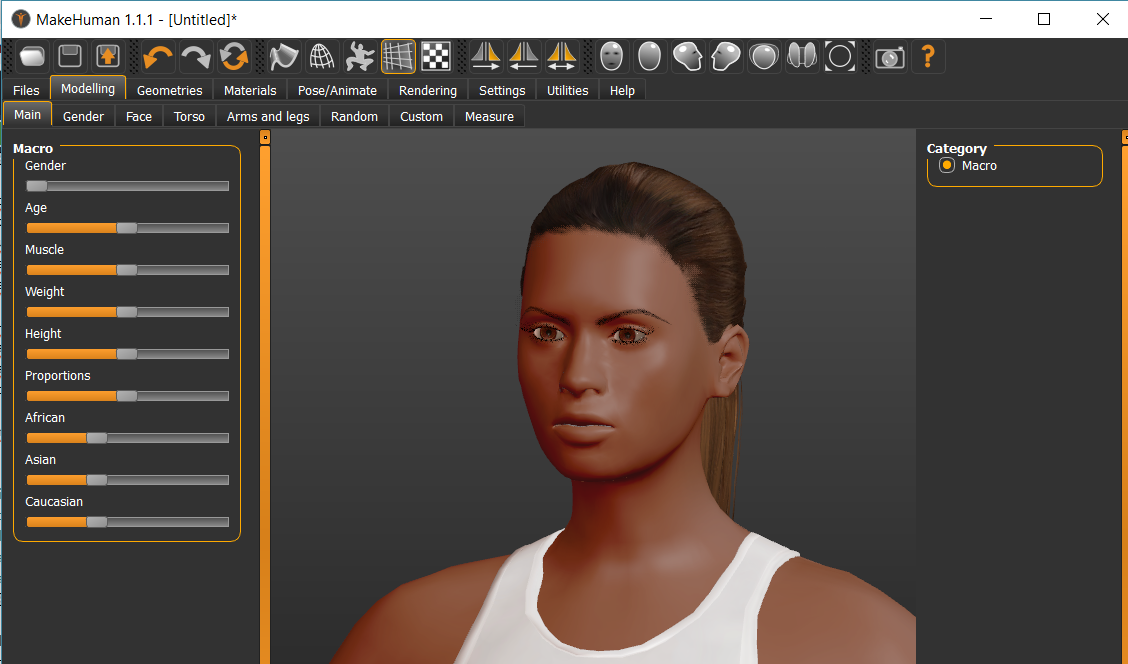
\includegraphics[width=0.6\columnwidth]{modele_existente/MakeHuman_main.png}
  \caption[Customizarea caracterului folosind MakeHuman]{Customizarea caracterului folosind MakeHuman\protect\footnotemark}
  \label{figure_1:picture_11}
\end{figure}

Ajustarea formei corporale este data de proportia intre picioare, maini si abdomen, precum si particulatizarea dimensiunii muschiilor pectorali, ai spatelui precum si altii. Un aspect interesant este dat de meniul special pentru maini care poate scala dimensiunea manii, lungimea degetelor, lungeamea podului palmei, diametrul degetelor si distanta intre degete.

Am decis ca Yuna sa fie o femeie in varsta de 25 de ani cu o inaltime de 180 de centrimetri. Alte particularitati speciale adaugate sunt: forma fetei care este ovala, muschii pectorali sunt cu putin mai dezvoltati.

I-am adaugat dinti si limba pentru a oferi mai multa viata caracterului. Acestea sunt vizibile doar atunci cand aceasta mimeaza cuvinte.

MakeHuman ne ofera posibilitatea de a imbraca caracterul la fel si pentru coafura, forma dintilor, forma sprancenelor, lungimea genelelor. Acestea pot sa fie descarcate de pe de pe site-ul comunitatii formate in jurul acestui proiect open source http://www.makehumancommunity.org/

Am ales din pachetul default peruca pe care o poarta, acesta este prins in coada. Prin intermediul comunitatii online am ales de asemenea bustiera, pantalonii si adidasii purtati de Yuna.

Cel mai important lucru care ne ajuta la animatii este ca alegem tipul de rig pe care il vom folosi pentru animatii. MakeHuman pune la dispozitie cinci modele de schelet. Eu am setat ca ea sa aiba scheletul default astfel proportia o sa fie buna intre calitatea animatiilor precum si memoria folosita in crearea acestor animmatii.

Un alt aspect tehnic foarte important este densitatea mesh-ei de pe caracter care variaza de la cel mai simplu la cel mai complex si sunt definite atat pentru caractere masculine si feminine.

\begin{figure}[th]
\centering
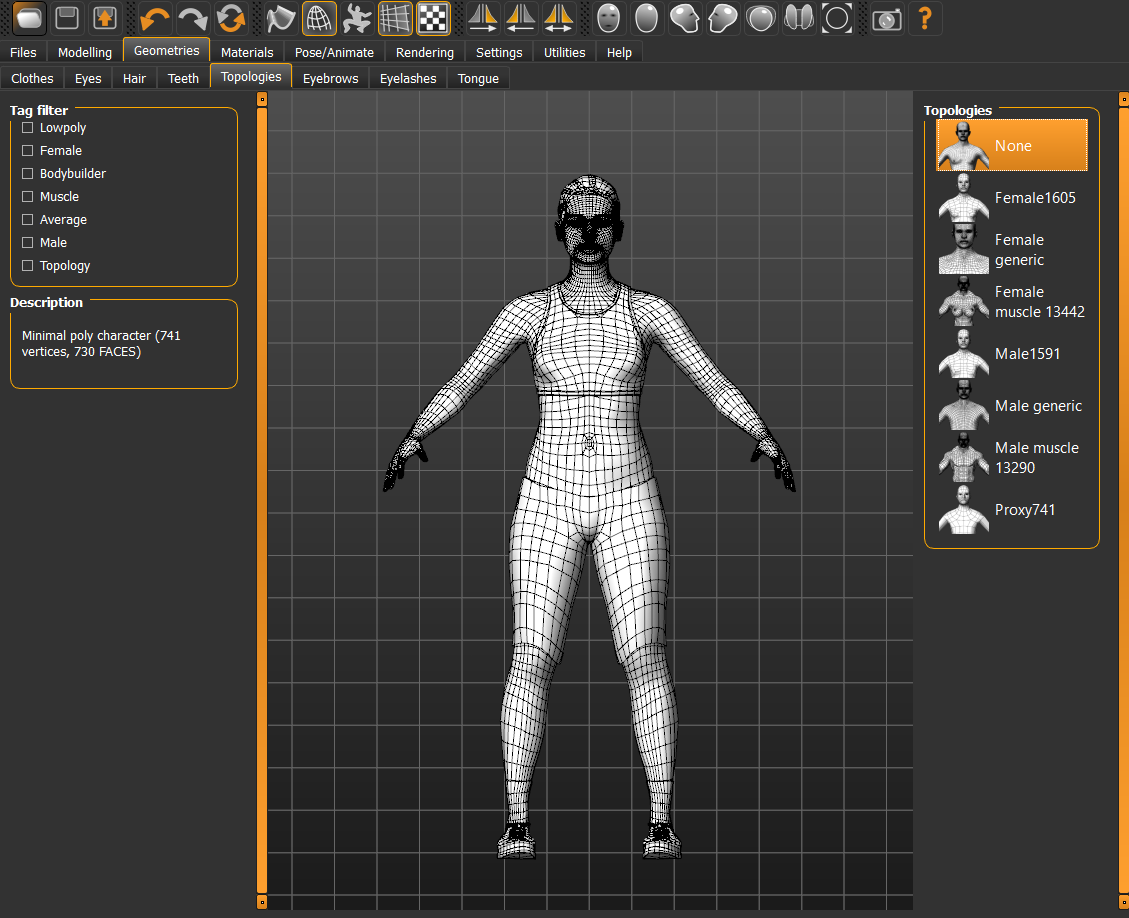
\includegraphics[width=0.6\columnwidth]{modele_existente/MakeHuman_meshDensity.png}
  \caption[Densitatea mesh-ei]{Densitatea mesh-ei\protect\footnotemark}
  \label{figure_1:picture_12}
\end{figure}

%%
%%  Scheletul
%%
\section{Scheletul}
Scheletul unui caracter este format dintr-o organizare ierarhica a oaselor pentru a se simula cat mai bine miscarile omenesti.

Scheletul este mandatoriu pentru crearea animatiilor pentru caractere tridimensionale. Aceste avatare sunt foarte folosite in jocurile video si in crearea filmelor.

Oasele digitale sunt organizate in relatie parinte-copil. Un exemplu in acest sens este miscarea umarului care va determina implicit miscarea bratului si al palmei.

Cu cat scheletul este format din mai multe oase cu atat se pot crea miscari mai detaliate, dar un dezavantaj este puterea necesara pentru randarea acestor animatii ceea ce duce la o gama foarte variata de schelete.

Exista o multitudine de forme de organizare al oaselor, dar caracterele care au acelasi schelet pot impartii animatii care au la baza scheletul respectiv.

Dupa cum am mentionat si in subcapitolul precedent, MakeHuman ne ofera posibilitatea de a aduga un schelet. Alegand scheletul inplicit vom avea ca elementul central al scheletului soldul. Yuna are scheletulul format de urmatoarele oase, avand aceasta ierarhie:

\begin{itemize}[noitemsep,topsep=0pt]
    \item sold - coloana - piept - umar - brat - antebrat - palma - degete
    \item sold - coloana - piept - gat - cap - fata
    \item sold - femur - gamba - picior
\end{itemize}

\begin{figure}[th]
\centering
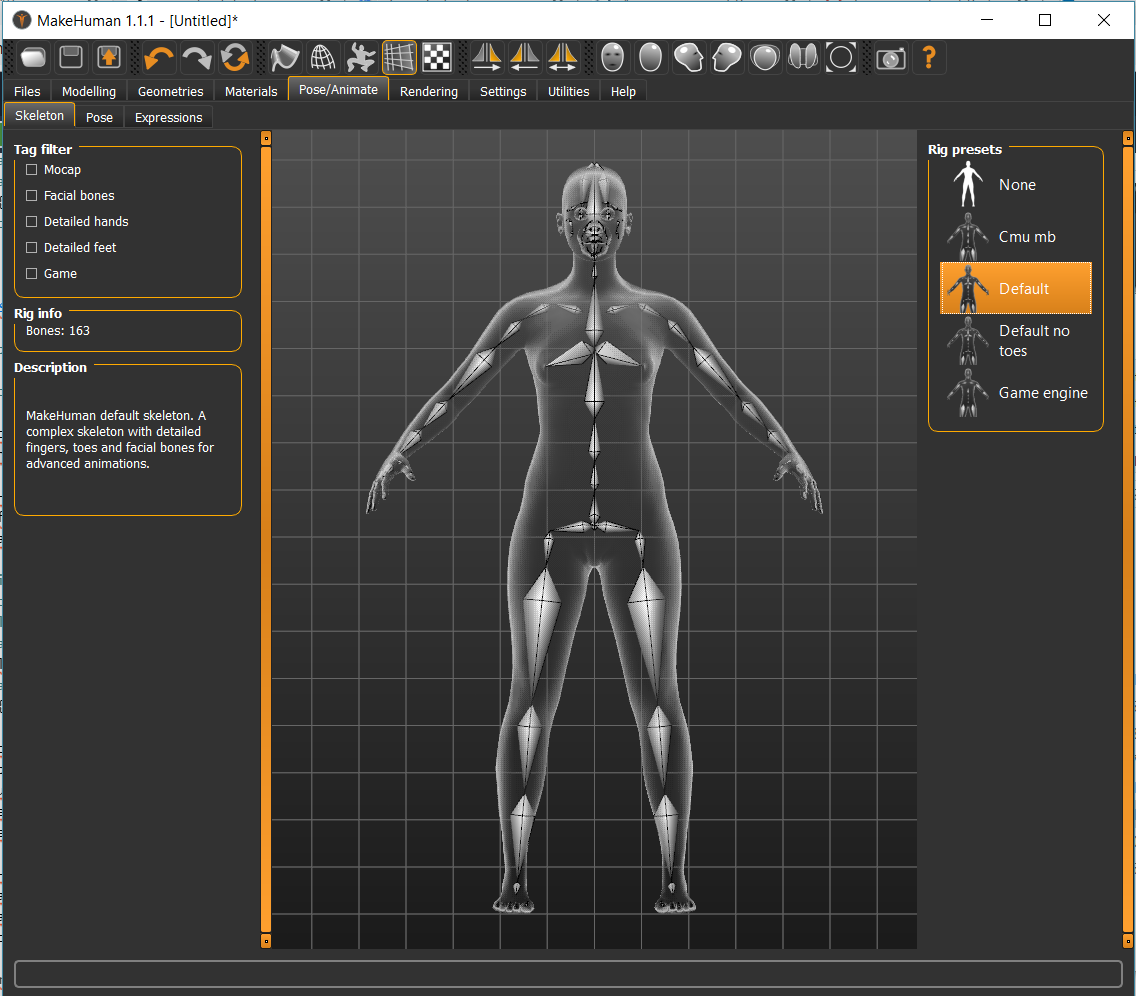
\includegraphics[width=0.6\columnwidth]{modele_existente/MakeHuman_Skeleton.png}
  \caption[Scheletul]{Scheletul\protect\footnotemark}
  \label{figure_1:picture_10}
\end{figure}


%%
%%  Animatii - Blender
%%
\section{Animatii - Blender}

Animatiile sunt folosite pentru aducerea la viata al obiectelor prin intermediul miscarilor fiind constituit dintr-o insiruire de cadrane de-a lungul unei cuante de timp. 

Animatiile pot fi create cu ajutorul diferitelor programe precum Blender, Maya ca apoi sa fie exporate in format FBX. De asemenea, este posibil sa se creeze in Unity, dar este mai complicat si nu este recomandat. Eu am ales sa folosesc Blender deoarece in al treilea an al facultatii l-am folosit pentru a realiza o tema la cursul de elemente de grafica pe calculator.

Cel mai important in cadrul unei animatii este avatarul. In cazul nostru, acest humanoid trebuie sa aiba:
\begin{itemize}
    \item structura oaselor
    \item mesh-ul
    \item maparea pe scheletului caracterului
\end{itemize}

Criteriile mentionate mai sus au fost indeplinite pentru antrenoarea virtuala, Yuna, cand am creat avatarul folosind MakeHuman. Acest avatar a fost exportat in format .MHX2 - MakeHuman eXchange format 2 care contine informatii mai importante despre mesh, materiale si scheletele suportate de MakeHuman. Acest format este dedicat transformatii caracterului din MakeHuman in Blender format

\begin{figure}[th]
\centering
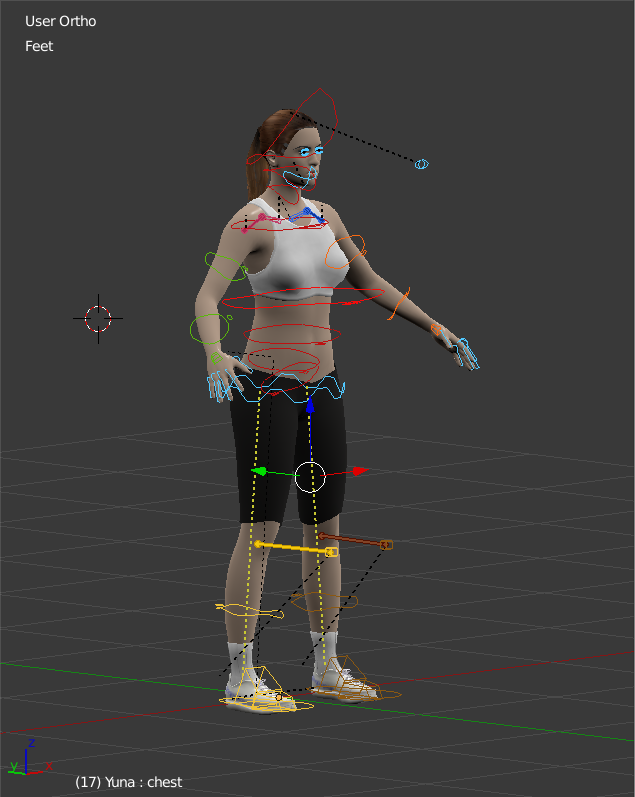
\includegraphics[width=0.3\columnwidth]{modele_existente/Blender_Animation1.png}
  \caption[Scheletul]{Scheletul\protect\footnotemark}
  \label{figure_1:picture_10}
\end{figure}

Pentru crearea exercitiilor am setat ca picioarele sa foloseasca Forward Kinematics pentru ca oasele sa fie ajustate.

Pentru crearea animatiilor tridimensionale, Blender ne ajuta in crearea acestora prin interpolarea a 2 cadre extreme. Cadrele cheie trebuie realizate de cei care vor sa creeze animatia. KeyFrame-urile sunt markere in timp care memoreaza coordonatele humanoidului. Frame-urile cheie reprezinta inceputul respectiv starsitul unor miscari line.

Pentru genoflexiuni a fost necesar sa creez doar trei cadrane cheie. Am decis ca animatia sa aiba 31 de cadre. In primul frame o avem pe Yuna in pozitia initiala (Fig. 12). Urmatorul frame este la 16 (Fig. 13) unde o surprinde pe Yuna la mijlocul exercitului; acest cadru cheie este important deoarece incepand cu acest cadru aceasta isi schimba directia. Pentru a oferi iluzia de ciclicitate al exercitiului ultimul frame este copia primului frame si acesta este pozitionata in cadrul 32 (Fig. 12). 

\begin{figure}[th]
\centering
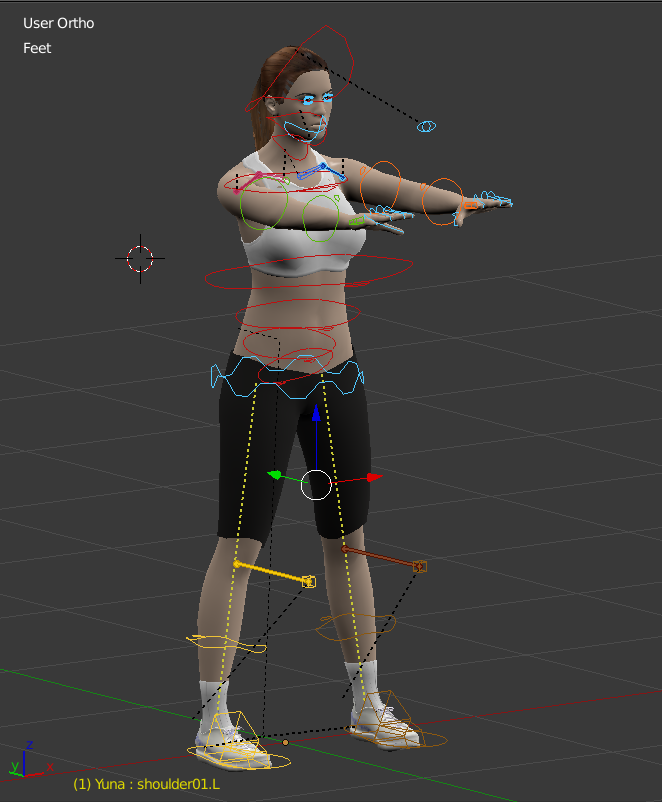
\includegraphics[width=0.3\columnwidth]{modele_existente/Blender_squatsFrame1.png}
  \caption[Scheletul]{Scheletul\protect\footnotemark}
  \label{figure_1:picture_10}
\end{figure}

\begin{figure}[th]
\centering
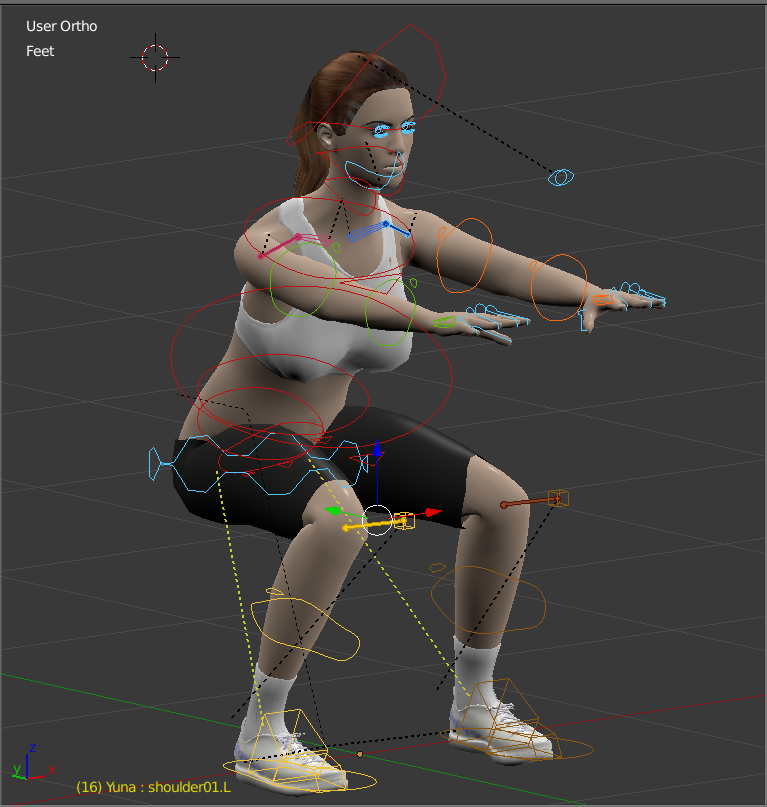
\includegraphics[width=0.3\columnwidth]{modele_existente/Blender_squatsFrame16.png}
  \caption[Scheletul]{Scheletul\protect\footnotemark}
  \label{figure_1:picture_10}
\end{figure}

% https://entertainment.howstuffworks.com/computer-animation1.htm

In momentul in care creem cadrele cheie totul este in spatiul normal de transformare. Aceste date sunt transformate in spatiul oaselor ceea ce restrictioneaza miscarile. 

In acest sens, osul central poate atat translata cat si roti pe cele trei axe tot arborele creat de oase. 

Nodurile care au parinte si au si copii au restrictia de a se roti. Oasele care fac parte din ultima categorie nu se pot translata deoarece este restrictionat de celelalte oase, atat parinte cat si copii. 

Ultimul tip este format din oasele care constituie frunze din structura ierarhica a oaselor si acestea fiind restrictionate la un capat nu se pot translata singura mutare posibila fiind rotatia.

Dupa ce s-au capturat frame-urile cheie trebuie sa "coacem" animatia. Prin acest lucru se intelege consolidarea animatiilor din sistemul nostru intr-o forma mai simplificata si permanenata. 

Dupa cum se poate sesiza, animatia are o multime de date care trebuie memorate precum: scheletul, mesh-ul precum si multitudinea de frame-uri fie definite prin cadre cheie fie cele determinate prin interpolarea a doua cadrane cheie.

Blender ne ofera posibilitatea de a coace ceea ce transforma cadranele provenite din interpolare cu cadrane cheie, astfel eliminam diferite dependinte. De asemenea, aceasta actiune previne dezintegrarea unor date. Cand am exportat-o pe Yuna am ales ca animatiile sa fie coapte la salvarea fisierului fbx.

%%
%%  Sala de fitness
%%
\section{Sala de fitness}

Am ales sa aleg game engine-ul Unity pentru createa spatiul de interactiune intre avatarul antrenoarei virtuale, Yuna, si utilizatorul aflat in perioada de recuperare sau pentru cei care vor sa isi mentina conditia fizica.

Sala de fitness contine:
\begin{itemize}
    \item o priveliste cu un lac
    \item pereti, perestre si tavan
    \item mingii gimnastice
    \item saltele de gimnastica
    \item haltere de diferite dimensiuni
    \item boxe
    \item antrenoarea virtuala
    \item corpuri de iluminat
    \item banca
\end{itemize}

\begin{figure}[th]
\centering
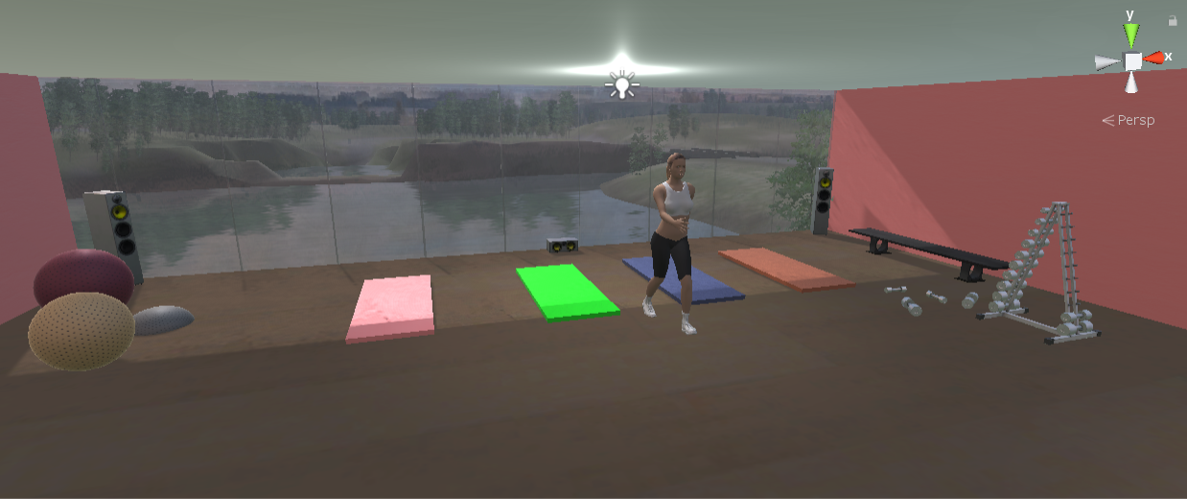
\includegraphics[width=1\columnwidth]{modele_existente/Unity_fitnessRoom.png} \caption[Scheletul]{Scheletul\protect\footnotemark}
  \label{figure_1:picture_10}
\end{figure}

Pentru crearea spatiului am ales sa folosesc asseturi aflate pe Unity store. Am ales o casa din care am ales back-ground-ul care este format dintr-un teren si un lac.

\begin{figure}[th]
\centering
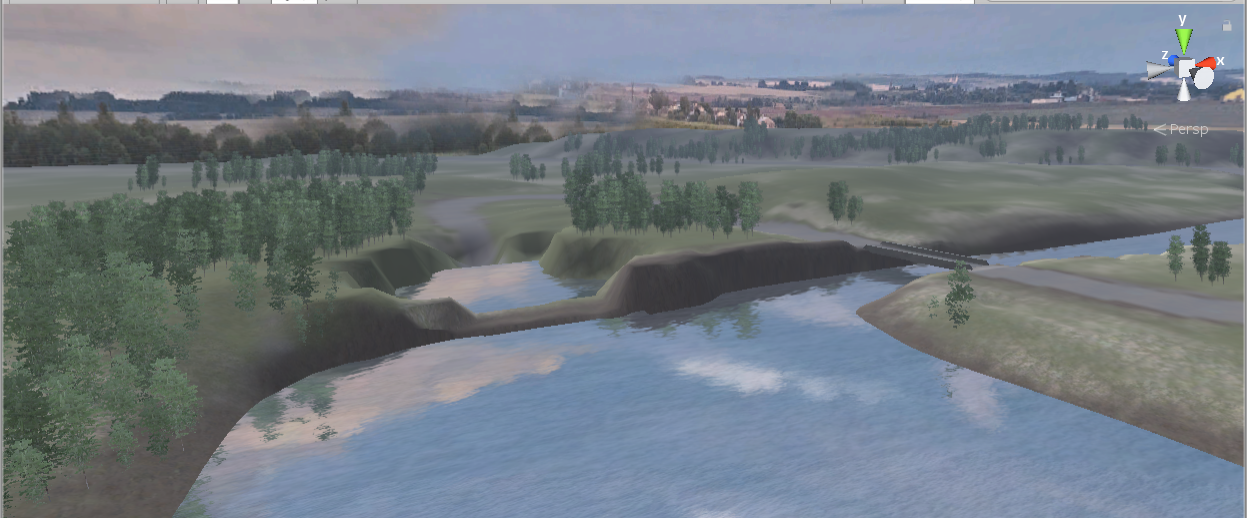
\includegraphics[width=1\columnwidth]{modele_existente/Unity_view.png}  \caption[Scheletul]{Scheletul\protect\footnotemark}
  \label{figure_1:picture_10}
\end{figure}

Pentru a crea camera am folosit cuburi pe care le-am redimensionat si pe care am adaugat o  textura gasita in asset store-ul oferit de Unity.

\begin{figure}[th]
\centering
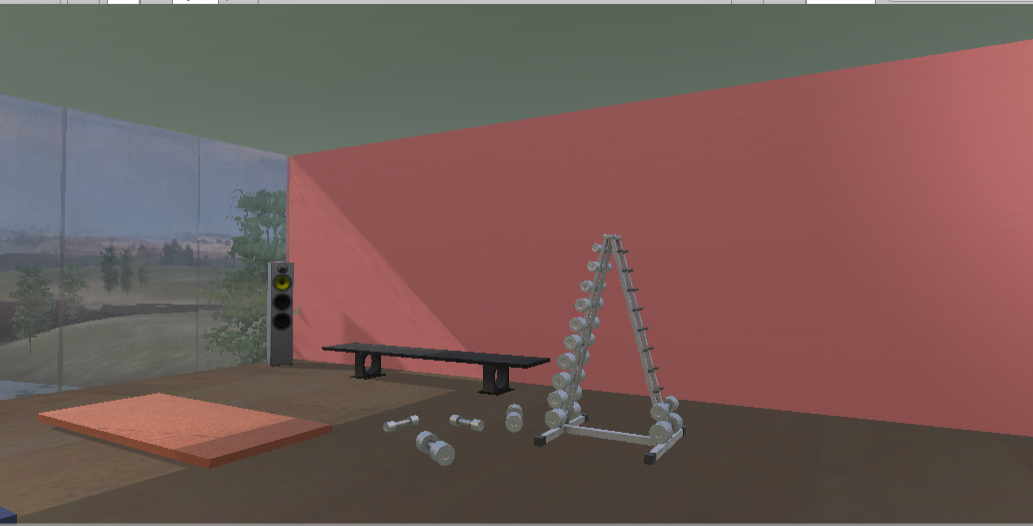
\includegraphics[width=1\columnwidth]{modele_existente/Unity_walls.png} \caption[Pereti]{Pereti\protect\footnotemark}
  \label{figure_1:picture_10}
\end{figure}

Ferestrele sunt cele gasite in pachetul care ofera mediul exteriul. Ferestrele permit trecerea luminii generate de soare

\begin{figure}[th]
\centering
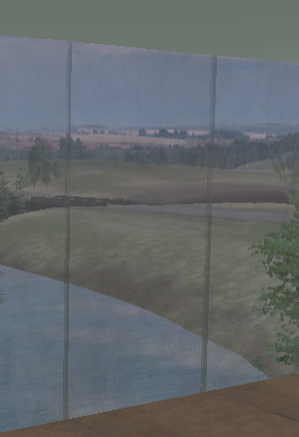
\includegraphics[width=0.33\columnwidth]{modele_existente/Unity_window.png} \caption[Ferestre]{Ferestre\protect\footnotemark}
  \label{figure_1:picture_10}
\end{figure}

Pentru mingiile gimnastice am creat sfere de diferite dimensiuni peste care am adaugat texturi care arata ca textura mingiilor din realitate

\begin{figure}[th]
\centering
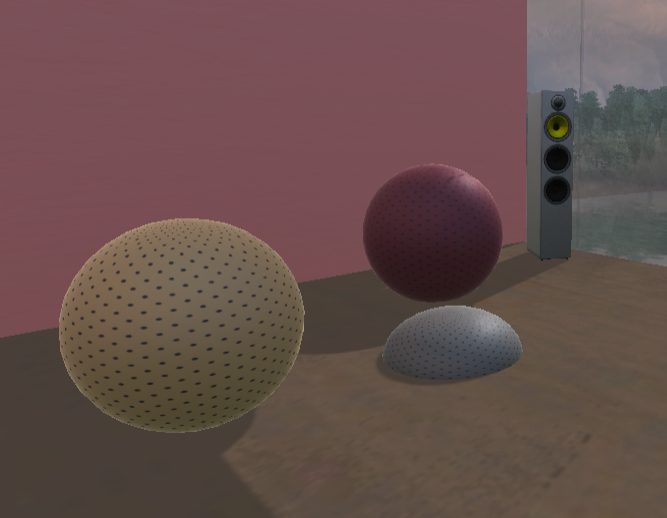
\includegraphics[width=0.6\columnwidth]{modele_existente/Unity_fitnessBalls.png} \caption[Mingii de gimnastica]{Mingii de gimnastica\protect\footnotemark}
  \label{figure_1:picture_10}
\end{figure}

\newpage
Saltele gimnastice au fost create in acelasi moduri ca mingiile gimastice. Am creat box-uri pe care le-am redimensionat. Peste acest meshe am adaugat texturi din acelasi pachet din care am luat texturile pentru mingi, pereti, tavan si podea.

\begin{figure}[th]
\centering
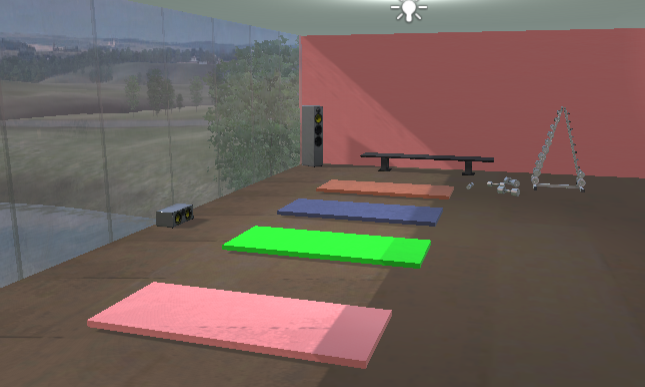
\includegraphics[width=0.9\columnwidth]{modele_existente/Unity_saltele.png} \caption[Scheletul]{Scheletul\protect\footnotemark}
  \label{figure_1:picture_10}
\end{figure}

\newpage

Am vrut sa simulez un mediu cat mai aproape de o sala de fitness de aceea am adaugat haltere care au fost gasit in asset store. Dupa cum se poate observa haltere au greutati diferite

\begin{figure}[th]
\centering
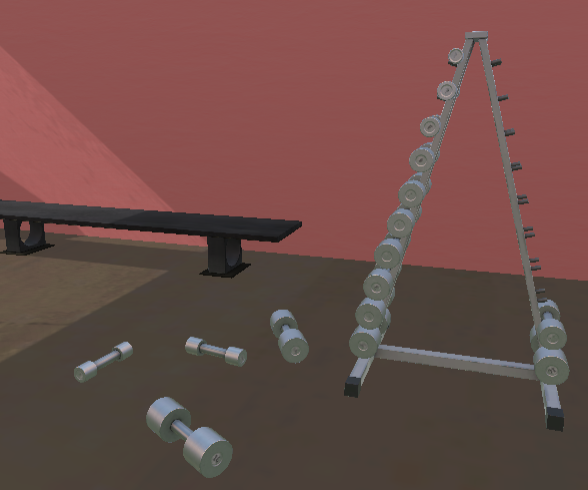
\includegraphics[width=0.6\columnwidth]{modele_existente/Unity_haltere.png} \caption[Scheletul]{Scheletul\protect\footnotemark}
  \label{figure_1:picture_10}
\end{figure}

Pentru a crea un mediu cat mai satisfacator si prielnic pentru antrenamete am adaugat boxe care au fost gasite in asset store.% In sectiuniea viitoare voi explica mai multe detalii legate de fundalul sonor.

\begin{figure}[th]
\centering
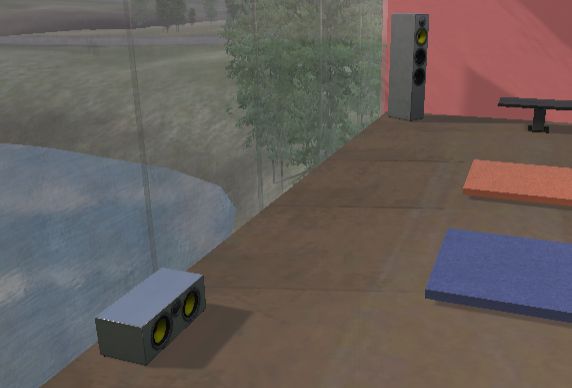
\includegraphics[width=0.6\columnwidth]{modele_existente/Unity_boxe.png} \caption[Scheletul]{Scheletul\protect\footnotemark}
  \label{figure_1:picture_10}
\end{figure}

%\todo[inline, color=blue!40]{}

%\begin{itemize}
%    \item antrenoarea virtuala
%    \item corpuri de iluminat
%    \item banca
%\end{itemize}

\newpage

%%
%%  Sala de fitness
%%
\section{Animatiile in modul de joc}

Pentru a crea animatiile din modul de joc a fost necesar sa creez un crontroller de animatii pe care l-am pus peste mesh, ceea ce a generat miscarile Yunei in game play.

In momentul acual am creat animatia pentru un exercitiu de ridicare ape rand al bratelor.

\begin{figure}[th]
\centering
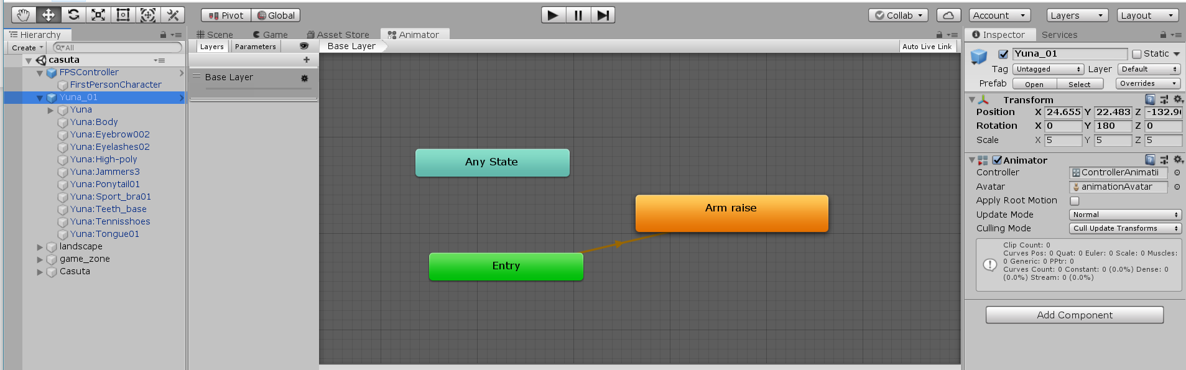
\includegraphics[width=1\columnwidth]{modele_existente/Unity_animationController.png} \caption[Scheletul]{Scheletul\protect\footnotemark}
  \label{figure_1:picture_10}
\end{figure}

%%
%%  Evaluare
%%
\chapter{Urmatorii pasi}

In perioada urmatoare imi propun sa folosesc 
\begin{enumerate}
    \item Kinect-ul pentru a captura miscarile userului. 
    \item Adaugarea mai multor controlere de animatiile care au deja in animatii realizare in blender
    \item adaugarea unei melodii de fundal
    \item crearea meniului
\end{enumerate}


%%
%%  Biografie
%%

\chapter*{Bibliografie}\addcontentsline{toc}{chapter}{Bibliografie}  
% * <marios.choudary@gmail.com> 2018-02-28T12:07:48.730Z:
% 
% > BIBLIOGRAFIE
% Am adaugat un paragraf cu cateva detalii despre folosirea citarilor bibliografice in Latex, despre folosirea lui "\cite" si despre posibilitatea folosirii bibliografiei si direct in fisierul Latex.
% 
% ^.

\begin{itemize}
	\item 	https://blender.stackexchange.com/questions/24633/what-is-the-difference-between-ik-and-fk-in-animation-on-blender
	\item 	https://docs.blender.org/manual/en/latest/index.html
	\item 	http://makehumancommunity.org
	\item 	https://docs.unity3d.com/Manual/UsingHumanoidChars.html
	\item   https://www.moddb.com/groups/anime/news/ubisoft-bets-wide
	\item   http://www.impulsegamer.com/360zumbafitnesscore.html
    \item   https://www.amazon.com/Biggest-Loser-Ultimate-Workout-Xbox-360/dp/B003S2SQFS5c
    \item   https://www.videogamesblogger.com/2010/11/16/ea-sports-active-2-walkthrough-video-guide-xbox-360-ps3-wii.htm
    \item   https://docs.blender.org/manual/en/latest/animation/index.html
    \item   https://cgcookie.com/articles/big-idea-baking
    \item   https://docs.unity3d.com/Manual/class-AnimatorController.html
    \item   https://www.microsoft.com/en-us/research/blog/stroke-recovery-gets-a-boost-from-kinect/
\end{itemize}


\end{document}